\textbf{P2)} El movimiento del pistón de un motor de automóvil se puede aproximar como un movimiento armónico simple (MAS).

Datos: la carrera (distancia total entre las posiciones extremas) es $0.100\ \mathrm{m}$, el motor funciona a $3500\ \mathrm{rev/min}$ y la masa del pistón es $0.450\ \mathrm{kg}$.

\begin{enumerate}[a)]
	\item Determine la aceleración máxima del pistón.
	\item Calcule la fuerza neta máxima que actúa sobre el pistón.
	\item Determine la rapidez máxima del pistón y su energía cinética máxima.
	\item ¿Qué potencia media se requiere para acelerar el pistón desde el reposo hasta su rapidez máxima?
	\item Repita los incisos (b), (c) y (d) si el motor funciona a $7000\ \mathrm{rev/min}$.
\end{enumerate}

\vspace{0.3cm}
\begin{center}
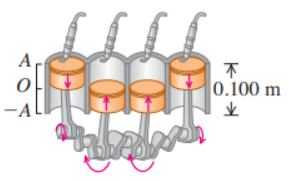
\includegraphics[width=0.32\textwidth]{imagenes/Ayudantia 7.PNG}
\end{center}
